% -*- latex -*-
%%%%%%%%%%%%%%%%%%%%%%%%%%%%%%%%%%%%%%%%%%%%%%%%%%%%%%%%%%%%%%%%
%%%%%%%%%%%%%%%%%%%%%%%%%%%%%%%%%%%%%%%%%%%%%%%%%%%%%%%%%%%%%%%%
%%%%
%%%% This text file is part of the source of 
%%%% `Parallel Programming in MPI and OpenMP'
%%%% by Victor Eijkhout, copyright 2012-6
%%%%
%%%% hybrid.tex : about hybrid computing
%%%%
%%%%%%%%%%%%%%%%%%%%%%%%%%%%%%%%%%%%%%%%%%%%%%%%%%%%%%%%%%%%%%%%
%%%%%%%%%%%%%%%%%%%%%%%%%%%%%%%%%%%%%%%%%%%%%%%%%%%%%%%%%%%%%%%%

So far, you have learned to use MPI for distributed memory and OpenMP
for shared memory parallel programming. However, distribute memory
architectures actually have a shared memory component, since each
cluster node is typically of a multicore design. Accordingly, you
could program your cluster using MPI for inter-node and OpenMP for
intra-node parallelism.

Say you use 100 cluster nodes, each with 16 cores. You could then
start 1600 MPI processes, one for each core, but you could also start
100 processes, and give each access to 16 OpenMP threads.

\begin{tacc}
In your slurm scripts, the first scenario would be specified \n{-N 100
-n 1600}, and the second as
\begin{verbatim}
#$ SBATCH -N 100
#$ SBATCH -n 100

export OMP_NUM_THREADS=16
\end{verbatim}
\end{tacc}

There is a third choice, in between these extremes, that makes
sense. A~cluster node often has more than one socket, so you could put
one MPI process on each \indexterm{socket}, and use a number of
threads equal to the number of cores per socket.

\begin{tacc}
The script for this would be:
\begin{verbatim}
#$ SBATCH -N 100
#$ SBATCH -n 200

export OMP_NUM_THREADS=8
ibrun tacc_affinity yourprogram
\end{verbatim}

The \indextermtt{tacc_affinity} script unsets the following variables:
\begin{verbatim}
export MV2_USE_AFFINITY=0
export MV2_ENABLE_AFFINITY=0
export VIADEV_USE_AFFINITY=0
export VIADEV_ENABLE_AFFINITY=0
\end{verbatim}
If you don't use \n{tacc_affinity} you may want to do this by hand,
otherwise \indextermtt{mvapich2} will use its own affinity rules.
\end{tacc}

\begin{figure}[ht]
  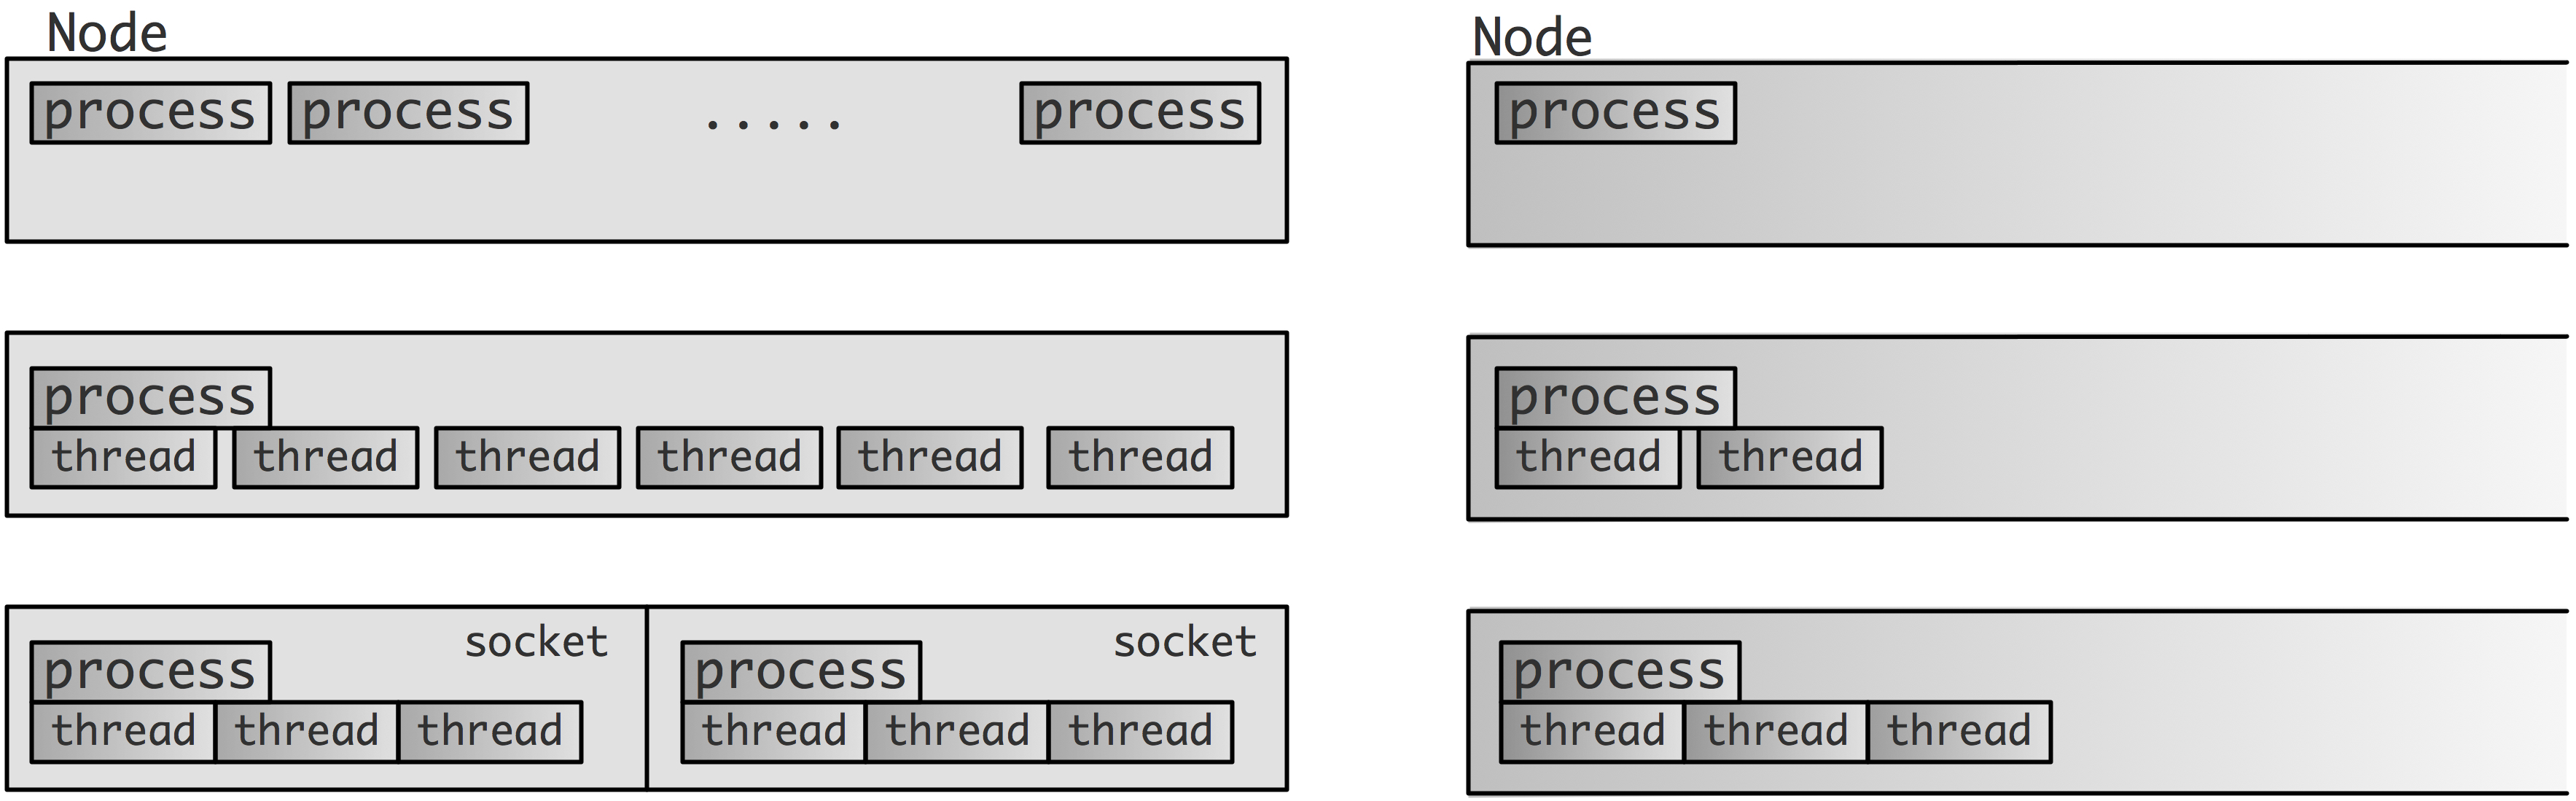
\includegraphics[scale=.13]{hybrid}
  \caption{Three modes of MPI/OpenMP usage on a multi-core cluster}
  \label{fig:hybrid-modes}
\end{figure}
%
Figure~\ref{fig:hybrid-modes} illustrates these three modes: pure MPI
with no threads used; one MPI process per node and full
multi-threading; two MPI processes per node, one per socket, and
multiple threads on each socket.

\Level 0 {Discussion}

The performance implications of the pure MPI strategy versus hybrid
are subtle.
\begin{itemize}
\item First of all, we note that there is no obvious speedup: in a
  well balanced MPI application all cores are busy all the time, so
  using threading can give no immediate improvement.
\item Both MPI and OpenMP are subject to Amdahl's law that quantifies
  the influence of sequential code; in hybrid computing there is a new
  version of this law regarding the amount of code that is
  MPI-parallel, but not OpenMP-parallel.
\item MPI processes run unsynchronized, so small variations in load or
  in processor behaviour can be tolerated. The frequent barriers in
  OpenMP constructs make a hybrid code more tightly synchronized, so
  load balancing becomes more critical.
\item On the other hand, in OpenMP codes it is easier to divide the
  work into more tasks than there are threads, so statistically a
  certain amount of load balancing happens automatically.
\item Each MPI process has its own buffers, so hybrid takes less
  buffer overhead.
\end{itemize}

\begin{exercise}
  Review the scalability argument for 1D versus 2D matrix
  decomposition in \HPSCref{sec:parallel-dense-mvp}. Would you get
  scalable performance from doing a 1D decomposition (for instance, of
  the rows) over MPI processes, and decomposing the other directions
  (the columns) over OpenMP threads?
\end{exercise}

Another performance argument we need to consider concerns message
traffic.  If let all threads make MPI calls (see
section~\ref{sec:init-thread}) there is going to be little
difference. However, in one popular hybrid computing strategy we would
keep MPI calls out of the OpenMP regions and have them in effect done
by the master thread.
%
In that case there are only MPI messages
between nodes, instead of between cores. This leads to a decrease in
message traffic, though this is hard to quantify. The number of
messages goes down approximately by the number of cores per node, so
this is an advantage if the average message size is small. On the
other hand, the amount of data sent is only reduced if there is
overlap in content between the messages.

Limiting MPI traffic to the master thread also means that no buffer
space is needed for the on-node communication.

\Level 0 {Recognizing shared memory in MPI}
\label{mpi-comm-split-type}

MPI's one-sided routines take a very symmetric view of processes:
each process can access the window of every other process (within a communicator).
Of course, in practice there will be a difference in performance
depending on whether the origin and target are actually
on the same shared memory, or whether they can only communicate through the network.
For this reason MPI makes it easy to group processes by shared memory domains
using \indexmpishow{MPI_Comm_split_type}.

\mpiRoutineRef{MPI_Comm_split_type}

In the following example, \n{CORES_PER_NODE} is a platform-dependent
constant:
%
\verbatimsnippet{commsplittype}

\Level 0 {Hybrid MPI-plus-threads execution}
\label{sec:init-thread}

In hybrid execution, the main question is whether all threads
are allowed to make MPI calls. To determine this,
replace the \n{MPI_Init} call by
%
\mpiRoutineRef{MPI_Init_thread}
%
Here the \n{required} and \n{provided} parameters can take the following
values:
\begin{description}
\item[\texttt{MPI\_THREAD\_SINGLE}]\indexmpi{MPI_THREAD_SINGLE} Only a
  single thread will execute.
\item[\texttt{MPI\_THREAD\_FUNNELLED}]\indexmpi{MPI_THREAD_FUNNELLED}
  The program may use multiple threads, but only the main thread will
  make MPI calls.

  The main thread is usually the one selected by the
  \indexpragma{master} directive, but technically it is the only that
  executes \indexmpishow{MPI_Init_thread}. If you call this routine in
  a parallel region, the main thread may be different from the master.
\item[\texttt{MPI\_THREAD\_SERIAL}]\indexmpi{MPI_THREAD_SERIAL} The
  program may use multiple threads, all of which may make MPI calls,
  but there will never be simultaneous MPI calls in more than one
  thread.
\item[\texttt{MPI\_THREAD\_MULTIPLE}]\indexmpi{MPI_THREAD_MULTIPLE}
  Multiple threads may issue MPI calls, without restrictions.
\end{description}

\begin{tacc}
  The \indexterm{mvapich} implementation of MPI
  does have the required threading support, but you need to set this environment variable:  
\begin{verbatim}
export MV2_ENABLE_AFFINITY=0
\end{verbatim}
  Another solution is to run your code like this:
\begin{verbatim}
  ibrun tacc_affinity <my_multithreaded_mpi_executable
\end{verbatim}
\end{tacc}

The \emph{mpirun}\index{mpirun!and environment variables}
program usually propagates \indexterm{environment variables},
so the value of \indextermtt{OMP_NUM_THREADS} when you call \n{mpirun}
will be seen by each MPI process.

\begin{itemize}
\item It is possible to use blocking sends in threads, and let the
  threads block. This does away with the need for polling.
\item You can not send to a thread number: use the MPI
  \indextermbus{message}{tag} to send to a specific thread.
\end{itemize}

\begin{exercise}
Consider the 2D heat equation and explore the mix of MPI/OpenMP
parallelism:
\begin{itemize}
\item Give each node one MPI process that is fully multi-threaded.
\item Give each core an MPI process and don't use multi-threading.
\end{itemize}
Discuss theoretically why the former can give higher performance.
Implement both schemes as special cases of the general hybrid case,
and run tests to find the optimal mix.
\end{exercise}

